%% XeLaTex

\documentclass[preprint,12pt,3p]{elsarticle}
\usepackage{amssymb}
\usepackage{caption}
\usepackage{graphicx, subfig}
\usepackage{algorithm,algorithmic}
\usepackage[BoldFont,SlantFont,CJKchecksingle]{xeCJK}
\setCJKmainfont[BoldFont=SimHei,SlantedFont=KaiTi]{SimSun}
\setCJKsansfont[BoldFont=SimHei,SlantedFont=KaiTi]{SimSun}
\setCJKmonofont[ItalicFont={Adobe Fangsong Std}]{SimSun}
\setCJKfamilyfont{zhhei}{Adobe Song Std}
\journal{Biologic Intelligence and Algorithm}

\begin{document}
\setlength{\baselineskip}{20pt}
\setlength\parindent{2em}
\begin{frontmatter}

\title{阴性选择算法研究}
\author{李美珍 11716026}
\address{农业与生物技术学院}
\ead{limeizhen@zju.edu.cn}

\begin{abstract}
阴性选择原理是免疫系统核心原理之一,参照该原理提出的阴性选择算法被广泛地应用于工程异常检测中。本文中,我们首先简要描述生物体中免疫细胞的阴性选择过程,由此引入阴性选择算法的模型和数学描述,并介绍这一算法自提出之后进行的几点优化。
\end{abstract}

\begin{keyword}
阴性选择算法 \sep 数学描述 \sep 匹配阈值 \sep 黑洞  
\end{keyword}

\end{frontmatter}

\section{生物体中的阴性选择过程}
\label{sec1}
生物体的免疫系统是一种复杂的自适应系统,其主要作用是识别体内所有细胞与分子,保护生物体不受外部病原体的侵害,其中的关键步骤就是区分“自我”和“非我”。免疫系统的模式识别本质上是抗体和抗原决定簇之间的互相匹配,其中抗体是指免疫细胞产生的可以识别并结合外来病原物的一种蛋白质,抗原决定簇是指能够免疫系统识别的并且可以与抗体结合的抗原分子的部分。相较抗体而言,抗原的概念较为宽泛,任何一种物质都可能被免疫系统当做抗原物质。当抗体识别结合自体抗原时,就会引发自身免疫反应,对机体产生损害。在生物体中,免疫系统通过免疫耐受来抑制自身免疫反应。
\par
免疫系统的免疫耐受主要通过T细胞实现,T细胞执行适应性细胞免疫应答,并辅助B细胞执行体液免疫应答。胸腺中包含了生物体的大多数自我抗原决定簇,T细胞在胸腺中成熟,所以在成熟期间,T细胞可以暴露给多数的自体抗原决定簇。如果一个未成熟T细胞由于结合自我抗原而激活,则会在胸腺中被清除;而那些存活的T细胞则继续发育成熟并离开胸腺,在机体中行使相应的免疫功能。因此,经过胸腺阴性选择过程的T细胞对于大多数的自我抗原都表现出耐受的特性。由于未被激活的T细胞才存活下来,所以该过程称为T细胞的阴性选择。

\section{阴性选择的算法分析}
\label{sec1}
\subsection{算法实现}
\label{subsec1}
阴性选择算法以免疫细胞阴性选择过程为原理,通过不断与自我集进行匹配,来获得区分“自我”和“非我”的能力。我们首先定义模型中抗原与抗体匹配的规则为部分匹配规则,实际应用中采用多种部分匹配实现阴性选择算法,如连续r位匹配规则、海明距离或者编辑距离等。经典的阴性选择算法过程如下:
\par
1. 定义自体S为长度等于l的字符串集合,即待保护的集合。
\par
2.定义部分匹配规则(包括匹配阈值r)、匹配阈值以及系统匹配失败率等参数。
\par
3.随机产生长度为l的字符串a;
\par
4.令a依次与自我集S中的自我元素相匹配,依据步骤2中所定义的匹配规则与匹配阈值判断a是否与自我集中元素匹配,若匹配则返回步骤3继续产生随机字符串进行匹配;若不与任何自我字符串匹配,则a成为有效检测器,加入成熟检测器集合R。(见Algorithm 1及Figure 1)
\par
5.通过不断地将R中的检测器与S比较来起到监控自我集变化、及时更新检测集的目的。
\par
6. 将待检测字符串与成熟检测器进行匹配,若符合匹配规则,则报告有害字符串。(见Algorithm 2及Figure 2)

\begin{algorithm}[H]
  \caption{生成成熟检测器}          
  \label{alg1}  
    \begin{algorithmic}  
       \STATE Input:SelfData
       \STATE Output:Repertoire
       \STATE Repertoire $\Leftarrow$ emptyset
       \WHILE {$ !StopCondition()$}
       \STATE Detectors $\Leftarrow$ GenerateRandomDetectors()
       \FOR {Detector[i] $\in$ Repertoire }
       \IF {$not$ Matches(Detector[i],SelfData)}
       \STATE Repertoire $\Leftarrow$ Detector[i]
       \ENDIF
       \ENDFOR
       \ENDWHILE
       \STATE Return (Repertiore)
   \end{algorithmic}
\end{algorithm} 

\begin{algorithm}[H]
 \caption{利用检测器进行监控}          
 \label{alg2}      
   \begin{algorithmic}  
      \STATE Input:InputSamples,Repertoire
      \FOR {Input[i] $\in$ InputSamples}
      \STATE Inputiclass $\Leftarrow$ nonself  
      \FOR {Detector[j] $\in$ Repertoire }
      \IF {Matches(Detector[j],SelfData)}
      \STATE Inputiclass $\Leftarrow$ self
      \ENDIF
      \ENDFOR
      \ENDFOR            
   \end{algorithmic}
\end{algorithm} 

\begin{figure}[hb]
  \centering
  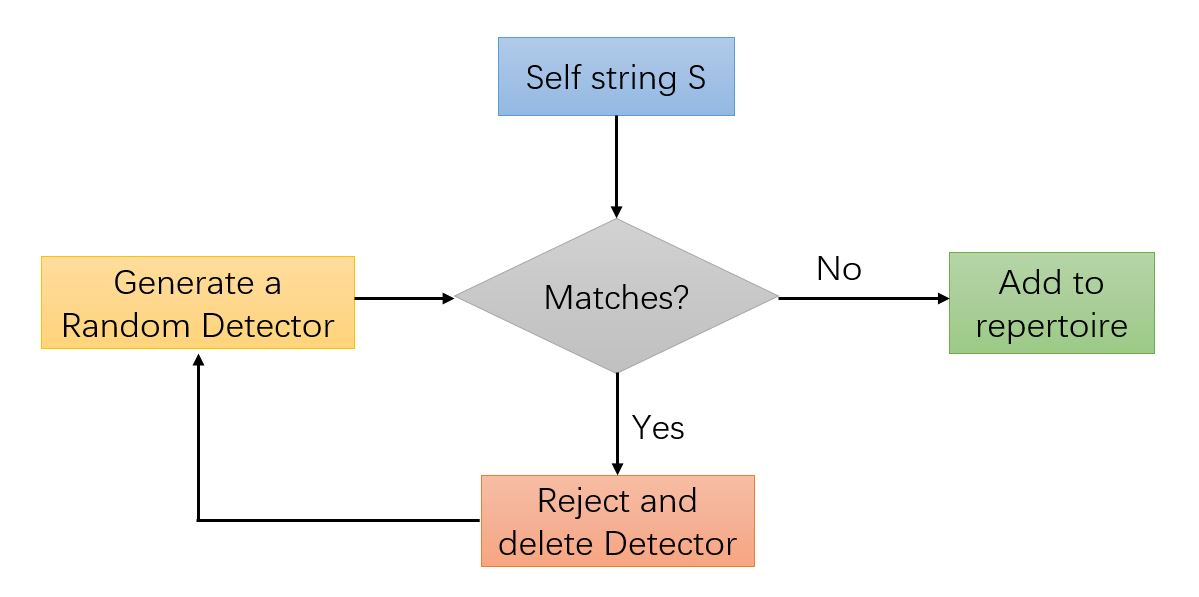
\includegraphics[width=0.8\textwidth]{img/NSAflowchart1.jpg}
  \caption{生成成熟检测器}
\end{figure}

\begin{figure}[hb]
  \centering
  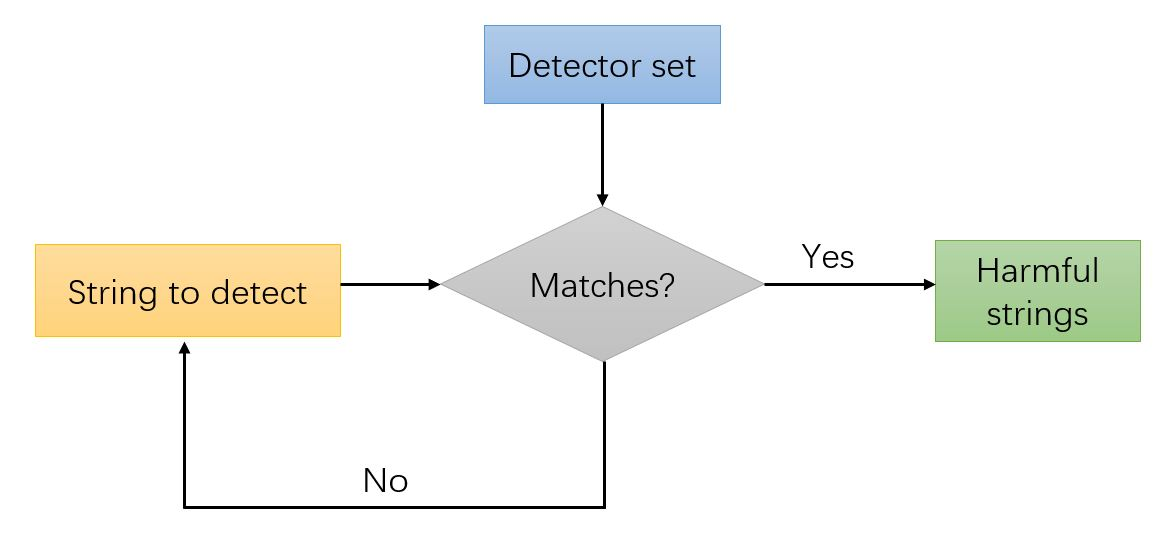
\includegraphics[width=0.8\textwidth]{img/NSAflowchart2.jpg}
  \caption{检测器用于监控}
\end{figure}

\subsection{数学描述}
\label{subsec2}
在这一节,我们定义一些基本的算法因素符号来推导一些理论上的公式,建立一个简单的阴性选择算法数学模型。我们给定以下参数:
\par
N$_{R_0}$:初始检测器数目
\par
N$_{R}$:成熟检测器集所具有的有效监测器数目 
\par
N$_{S}$:自我集中自我元素数目
\par
P$_{M}$:两个随机字符串在特定匹配规则下的匹配概率
\par
P$_{f}$:系统匹配失败率
\par
f:一个随机字符串不与任何自我集中的元素匹配的概率
\par
那么一个随机字符不与一个自我元素匹配的概率是(1-P$_{M}$),所以一个随机字符串不与任何自我集中元素匹配的概率,即一个随机字符串成为有效监测器的概率为:
\begin{equation}
    f=(1-P_{M})^{N_{S}}
\end{equation}

\par
如果一个随机字符不与任何一个有效监测器匹配即为系统匹配失败,那么系统匹配失败率是:
\begin{equation}
    P_f=(1-P_{M})^{N_{R}}
\end{equation}

\par
在特定的系统匹配失败率的要求下,成熟监测器所具有的有限检测器的数目为:
\begin{equation}
    N_R=\frac{lnP_f}{ln(1-P_M)}
\end{equation}

\par
那么,生成足够数目的有效检测器时所需要的迭代次数为:
\begin{equation}
    Iterations:D=\frac{lnP_f}{(1-P_{M})^{N_{S}}ln(1-P_M)}
\end{equation}

\section{阴性选择算法的优化}
\label{sec1}
\subsection{对检测器生成算法的优化}
\label{subsec1}
由公式(4)可知,在系统匹配失败率等参数确定的条件下,生成成熟检测器的迭代次数与自我集元素个数成指数关系。这样的模型难以解决自我集较大的复杂问题。针对基于连续r位匹配规则的有效检测器生成,有两种高效的检测器生成算法,分别是线性时间检测器算法和贪婪检测器生成算法。这两种算法都会首先剔除有效检测器中不可能含有的模式串子片段,以剩余的模式串片段建立一个部分模式串库,然后通过对模式串片段进行补充和组合来生成随机选取的有效检测器。经过优化,生成成熟检测器的算法时间复杂度与自我集规模呈线性关系。
\par
线性时间检测器生成算法的时间复杂度为:
\begin{equation}
    TimeComplexity=O((l-r)\times{N_S})+O((l-r)\times{2^r})+O(l\times{N_R})
\end{equation}
\par
贪婪检测器生成算法的时间复杂度为:
\begin{equation}
    TimeComplexity=O((l-r)\times{N_S})+O((l-r)\times{2^r}\times{N_R})+O(l\times{N_R})
\end{equation}


\subsection{对检测过程时间复杂度的优化}
\label{subsec2}
检测器检测异常值过程的时间复杂度与有效监测器个数呈线性相关,由公式(3)可知,在系统匹配失败率确定的前提,有效监测器的个数与匹配规则有关。之前我们将匹配规则定义为部分匹配规则。在这里我们分析两个重要的部分匹配规则。
\begin{figure}[hb]
  \centering
  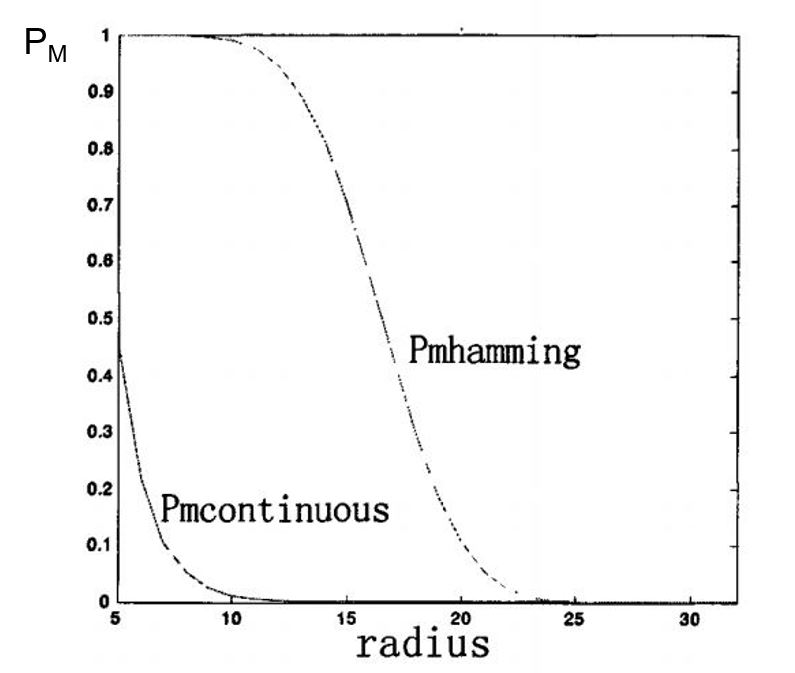
\includegraphics[width=0.5\textwidth]{img/CompareCH.jpg}
  \caption{P$_{Mcontinous}$和P$_{Mhamming}$的比较}
\end{figure}

\par
连续r位匹配:两个长度为l的二进制串a、b,当且仅当它们在r或多于r个连续位上有相同字符时,它们在连续r位匹配规则下匹配。两个长度为l的随机字符串在连续r位匹配规则下匹配的概率为:
\begin{equation}
   P_Mcontinous \approx \frac{1}{2^r}[\frac{l-r}{2}+1]
\end{equation}
\par
海明距离匹配:两个长度为l的二进制串a、b,当且仅当它们在r或多于r个位置上有相同字符时,它们在海明距离匹配规则下匹配。两个长度为l的随机字符串在海明距离匹配规则下匹配的概率为:
\begin{equation}
   P_Mhamming = \frac{1}{2^r}\sum_{i=r}^{n}C_l^i
\end{equation}

\par
在给定的匹配阈值r的前提下,海明距离规则的匹配概率要大于连续r位匹配规则,即采用海明距离匹配规则可以大大减少有效检测器的个数(见Figure 3)。但是在实际问题中,海明距离匹配规则并不是在所有问题中都推荐的,其在减少检测时间的情况下,会付出检测可靠性的代价,所以需要根据实际问题进行选择。


\subsection{对于黑洞问题的优化}
\label{subsec3}
在传统的阴性选择算法中,由于采用部分匹配规则,匹配阈值通常小于字符串长度,在检测过程中不可避免会产生黑洞问题(见Figure 4)。也就是说存在一个非我模式串a不能被任何一个检测器识别,即定义a为黑洞。
\begin{figure}[hb]
  \centering
  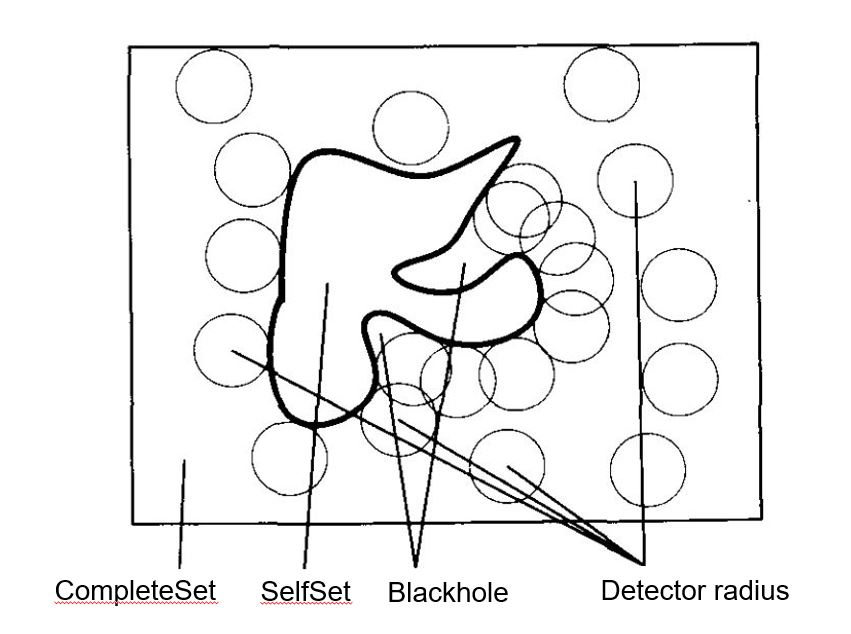
\includegraphics[width=0.6\textwidth]{img/blackhole.jpg}
  \caption{对于黑洞的定义} 
\end{figure}

\par
在生物免疫系统中也存在黑洞的问题,而且病原体倾向于向黑洞进化来逃避免疫应答。黑洞的存在取决于模式集的结构和匹配规则。自我模式越相似,黑洞数量越少;采用同一匹配规则,匹配阈值越大,黑洞数量越少。当匹配阈值r=l时,则匹配范围变成一个点,此时没有黑洞存在。但是在时间复杂度和检测灵敏度的要求下,实际情况中这种状态是不被允许的。为了减少黑洞数量,提出了r可变的检测器产生算法(见算法3)。设置匹配阈值变化为r$_{1}$<r$_{2}$<r$_{3}$<...<r$_{C}$。算法描述如下:
\par
1. 定义自体长度为l的自我集S。
\par
2. 随机产生一长度为l的字符串a。
\par
3. 将字符串a一次与S中的字符串匹配。
\par
4. 根据匹配规则,如果a不与S中任何字符串匹配,则a成熟,将a与匹配阈值加入到成熟检测器集中,转到第2步。
\par
5. 当a遇到与之匹配的字符串,将匹配阈值依次调整,记为为r$^{'}$,如果r$^{'}$>r$_{C}$,转到第2步,否则转到第3步。

\begin{algorithm}[H]
   \caption{r可变的阴性选择算法}          
   \begin{algorithmic}  
       \STATE Step1: Define SelfSet S (length=l) r$_1$,r$_2$,...,r$_c$
       \STATE Step2: a $\Leftarrow$ GenerateRandomString (length=l) r=r$_1$
       \STATE Step3: Matches (a,S[i])
       \IF {$not$ Matches(a,S[i])}
       \STATE go to step2
       \ELSIF {r \textgreater r$_c$}
       \STATE go to step2
       \ELSE
       \STATE r=r$_{++}$ 
       \STATE go to step3
       \ENDIF 
   \end{algorithmic}
\end{algorithm} 

\par
r可变的阴性选择算法核心思想是通过调整匹配阈值这一比较简单的方法来大幅降低黑洞数量(见Figure 5)。

\begin{figure}[hb]
  \centering
  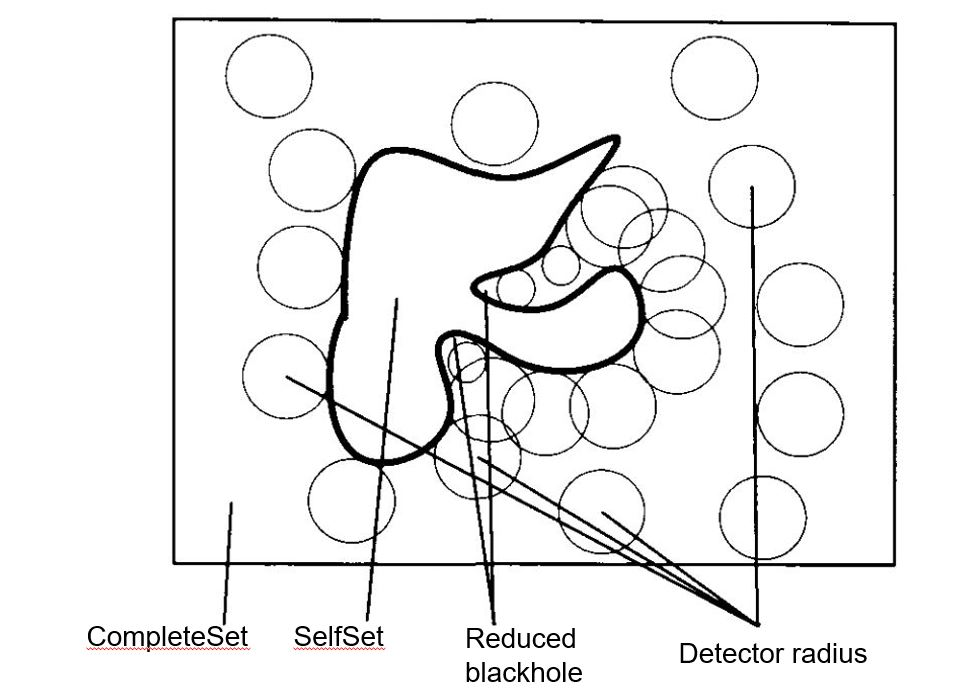
\includegraphics[width=0.6\textwidth]{img/reducedblackhole.jpg}
  \caption{优化之后黑洞数量减少}
\end{figure}

\par
和传统的阴性选择算法相比,r可变的阴性选择算法生成的检测器黑洞数量更少,生成检测器的迭代次数也变少,除此之外,二者还具有以下几点不同:
\par
(1)r可变的阴性选择算法有多个可调的匹配阈值,传统的阴性选择算法只有固定的匹配阈值。
\par
(2)r可变的阴性选择算法的检测器集中不仅有检测器,还包括与之对应的匹配阈值,传统的阴性选择算法只有检测器。
\par
(3)r可变的阴性选择算法产生的不同检测器检测范围不同,传统的阴性选择算法产生的不同检测器范围固定。
\par
也就是说,传统的阴性选择算法可以看做是r可变的阴性选择算法的一个特例。


\section{总结}
\label{sec4}
作为人工免疫系统的核心算法之一,阴性选择算法在计算机病毒检测、工具测损以及时间序列异常检测等方面都有广泛应用。其检测快速准确,且不需要关于异常的先验知识。本文介绍了阴性选择算法的生物学模型和数学描述,对于传统的阴性选择算法来说,其检测集与自我集规模呈指数关系,且检测黑洞数量较大,不能满足多数情况下对检测算法的要求。对其进行性能改进,对系统具有重要意义。为了降低时间复杂度、降低黑洞数量、提高检测率,本文总结了针对性的三个方面的改进,改进之后,产生检测器的时间消耗、黑洞数量、检测过程时间消耗均明显减少。
\end{document}


